\documentclass[12pt, twoside]{article}
\usepackage[francais]{babel}
\usepackage[T1]{fontenc}
\usepackage[latin1]{inputenc}
\usepackage[left=3mm, right=3mm, top=3mm, bottom=3mm]{geometry}
\usepackage{float}
\usepackage{graphicx}
\usepackage{array}
\usepackage{multirow}
\usepackage{amsmath,amssymb,mathrsfs}
\usepackage{soul}
\usepackage{textcomp}
\usepackage{eurosym}
 \usepackage{variations}
\usepackage{tabvar}
\usepackage{lscape}


\pagestyle{empty}

\begin{document}




\section*{\center{Devoir maison 7}}


\enskip





\fbox{

\begin{minipage}{18cm}
\textit{Devoir � rendre pour le \textbf{mercredi 11 mai 2011}. La partie
``coloriage'' de l'exercice 5 et l'exercice 6 sont � faire sur la photocopie.}
\end{minipage}
}





\ul{Exercice 1}

Les r�sultats de chacun de ces �l�ves sont-ils justes? Justifier vos r�ponses.

\begin{center}
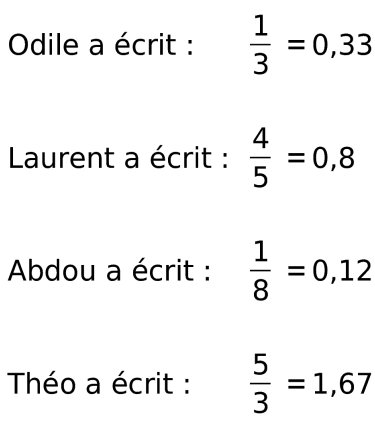
\includegraphics[width=35mm]{images/ex1.jpg} 
\end{center}

\bigskip

\ul{Exercice 2}


Recopier et compl�ter le tableau. Justifier chacune de vos r�ponses.


\enskip


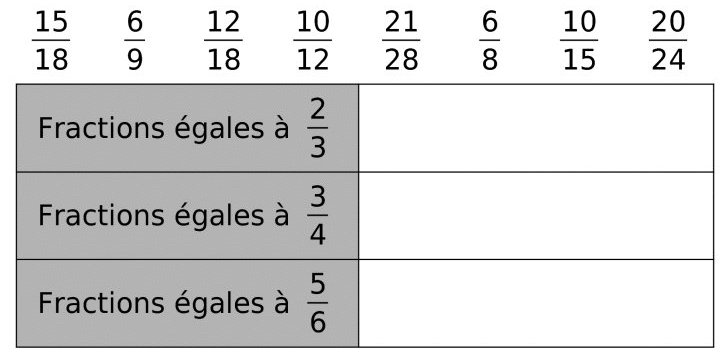
\includegraphics[width=6cm]{images/ex2.jpg}

\bigskip

\ul{Exercice 3}

Alexandre s'entraine pour une comp�tition de v�lo-cross. Il commence en for�t,
en mont�e sur une distance �gale � deux septi�mes du parcours, puis en descente
sur les quatre cinqui�mes de la distance restante. Il effectue la fin du
parcours le long d'une rivi�re.

\begin{enumerate}
  \item Recopier et compl�ter le sch�ma en coloriant les segments
  correspondants � chaque partie du parcours d'Alexandre (en rouge pour la
  mont�e, vert pour la descente et bleu pour la partie le long de la rivi�re):
  

  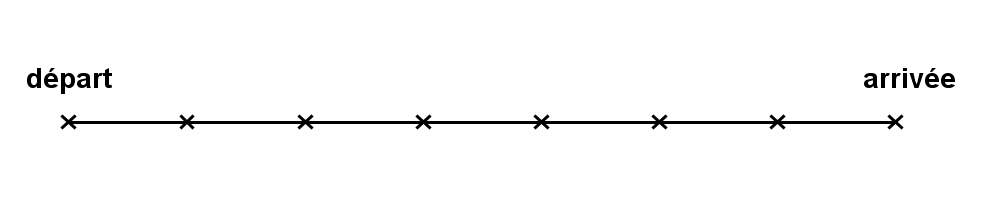
\includegraphics[width=75mm]{images/ex3.png} 








  \item  A quelle fraction de la longueur totale parcourue correspond la
  partie en descente?
   \item  A quelle fraction de la longueur totale parcourue correspond la
   partie le long de la rivi�re?  
\end{enumerate}

\bigskip


\ul{Exercice 4}



\begin{enumerate}
\item Tracer une demi-droite gradu�e en choisissant 
astucieusement une unit� de
longueur pour pouvoir placer facilement les points A d'abscisse $\dfrac{5}{6}$,
B d'abscisse $\dfrac{7}{6}$ et C d'abscisse $2+\dfrac{1}{6}$.
\item Quels sont les abscisses des milieux des segments [AB], [AC] et [BC]?
\end{enumerate}

\bigskip



\ul{Exercice 5}

On remplit un verre de 30 cl avec:
$\dfrac{1}{6}$ de jus d'orange; $\dfrac{3}{10}$ de jus de raisin;
$\dfrac{2}{5}$ de jus de pomme et le reste de jus de mangue.
\begin{enumerate}
  \item \begin{enumerate}
          \item Calculer la quantit�  de jus d'orange.
          \item Calculer la quantit� de jus de raisin.
          \item Calculer la quantit� de jus de pomme.
          \item Calculer la quantit� de jus de mangue.
\end{enumerate}

\item  Le rectangle ci-dessous repr�sente le verre.



\begin{enumerate}
  \item Colorier en vert la partie correspondant au jus d'orange, en rouge
  celle correspondant au jus de raisin et en vert celle correspondant au jus de
  pomme.
  \item A l'aide du dessin, donner la fraction repr�sentant le jus de mangue
  dans le verre.
  \item Calculer la quantit� de jus de mangue.
\end{enumerate}
\end{enumerate}






\begin{center}
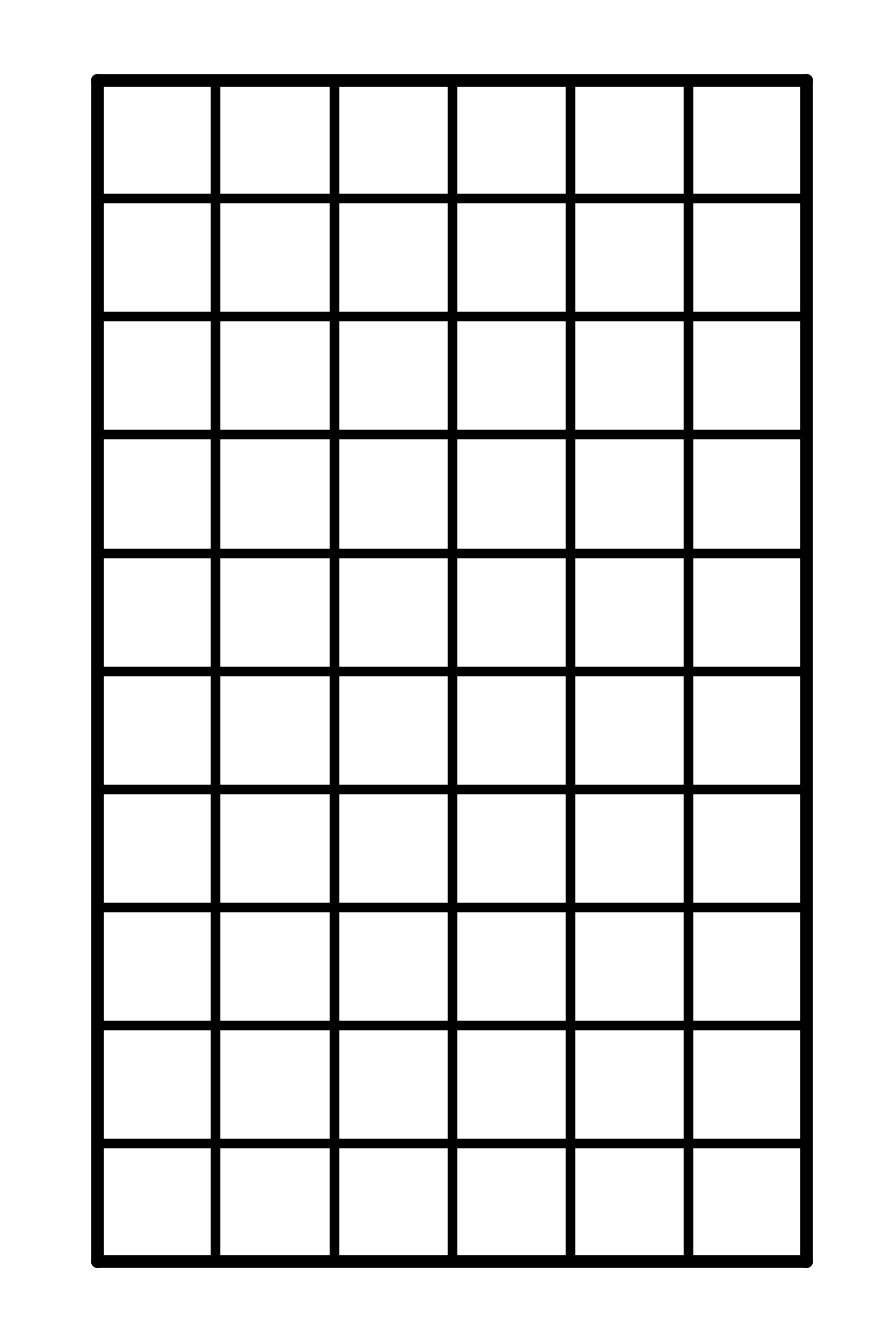
\includegraphics[width=25mm]{images/ex5.png} 
\end{center}

\bigskip

\ul{Exercice 6}

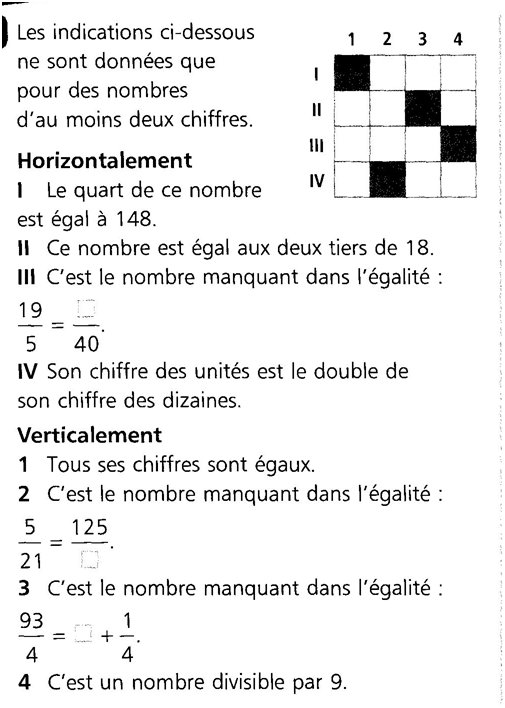
\includegraphics[width=70mm]{images/ex6.jpg} 

Justifier vos r�ponses sur votre copie.

\end{document}
